\begin{enumerate}
	\item L'administrateur se connecte au site avec ses identifiants. 
	\item Un nouveau bouton de navigation apparait dans la barre de navigation. 
	\item L'administrateur clique sur le bouton \textit{Admin}
	\item Il sélectionne \textit{Type Session} dans le menu déroulant. 
	\item L'administrateur atterrit sur la page de gestion des types de sessions. 
	\item Il clique sur le bouton edit
	\item Un formulaire apparait et il le remplit avec les bonnes informations (jour - heure [hh:mm])
	\item Il clique sur \textit{ok} 
\end{enumerate}

\vspace{\baselineskip}
\begin{figure}[h]
	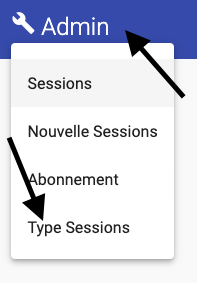
\includegraphics[width=0.4\textwidth,center]{Figures/us13-1}
	\caption{Menu de l'administrateur}
\end{figure}

\newpage
\begin{figure}[h]
	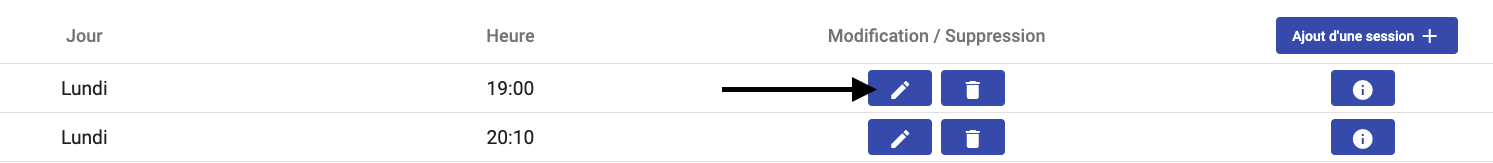
\includegraphics[width=0.9\textwidth,center]{Figures/us13-2}
	\caption{Bouton de modification du type de session}
\end{figure}

\vspace{\baselineskip}
\begin{figure}[h]
	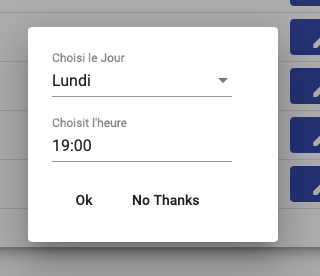
\includegraphics[width=0.4\textwidth,center]{Figures/us13-3}
	\caption{Formulaire de modification du type de session}
\end{figure}

\subsubsection{Gestion des erreurs}
	\paragraph{}
		Chaque type de session est unique, si l'administrateur rentre des informations correspondant à un type de session deja existant, une erreur apparaitra au dessus du formulaire.
	
\subsubsection{Diagramme de séquence}
	\paragraph{}
		Le diagramme de séquence de la modification d'un type de session est identique à celui de la création de session. Seule la première méthode appelé dans le backend change pour devenir \textit{editTypeSession}. 

\subsubsection{Scripts concernés}
	\begin{itemize}
		\item \Href{https://github.com/victorsmits/Aquabike/blob/master/backend/src/Controller/API/RegistrationControllerApi.php}{RegistrationControllerApi.php}
		\item \Href{https://github.com/victorsmits/Aquabike/blob/master/backend/src/Entity/TypeSession.php}{TypeSession.php}
		\item \Href{https://github.com/victorsmits/Aquabike/blob/master/frontend/src/app/type-session/edit-type-session.component.ts}{edit-type-session.component.ts}
		\item \Href{https://github.com/victorsmits/Aquabike/blob/master/frontend/src/app/type-session/edit-type-session.component.html}{edit-type-session.component.html}
	\end{itemize}
